%% LaTeX2e class for student theses
%% sections/content.tex
%% 
%% Karlsruhe Institute of Technology
%% Institute for Program Structures and Data Organization
%% Chair for Software Design and Quality (SDQ)
%%
%% Dr.-Ing. Erik Burger
%% burger@kit.edu
%%
%% Version 1.3.5, 2020-06-26

\chapter{Basic Concepts}
\label{chap:basics}

\textit{In this chapter we will go over some of the more fundamental concepts which are necessary to understand how explainers work in general and their challenges. Expert readers may skip this chapter.}

\section{Interpretability}

Interpretability is a rather vague concept which can be summarized in following statement: \enquote{can the average human understand it?}. This simple statement has multiple issues.
It is very unclear what that means in practice. A lot of work has been done to define that statement in the last few years \cite{lipton2017mythos}. The latter reference defines a few desiderata which models should have to be interpretable. We will go over some of them and explain what that means in our context of text classifiers.

\begin{itemize}
    \item \textbf{Simulatability}: In opposition to the opacity of artificial neural networks, simulatability is a property interpretable models need to have. The idea is, that a model is simulatable, if a person can contemplate the entire model at once in a \textit{reasonable} timeframe. This is important because it is possible to contemplate parts of artificial neural networks, and understand them because in itself they are very simple functions, but in such quantities, that it is impossible to contemplate them all at once. It also contradicts the idea that linear models are always interpretable. If complex enough, even a linear model is not humanly understandable.
    \item \textbf{Decomposability}: States that the model can be decomposed in parts which can be understood by themselves, without needing to understand the whole function. This notion of interpretability while being popular is controversial, because it excludes many models from being interpretable but I will make the argument that it is very much true. Humanly understandable means that one human can explain the model to another human. That is only possible if you can start somewhere, if you can put your explanation in logical following parts. This is how humans arguments, pick up information, a process called \textbf{active learning} \cite{activeLearning}. While a model might seem simple enough to be understood by the human mind, it needs to be decomposable so that a human can acquire the knowledge about the model in a structured way.
    \item \textbf{Algorithmic transparency}: While it is possible to understand how an algorithm works, it can be much more difficult to accept that the algorithm will provide the desired result. This is however an important part of Interpretability, if the algorithm cannot be trusted to work as intended, it is not really understood because the results are much more difficult to predict \cite{lipton2017mythos}.
\end{itemize}


Let's now analyze what that means in the case of text classification using artificial neural networks. It is obvious that we cannot provide any of the three desiderata for modern neural networks. It is thus necessary to take a detour to try to explain the model in an interpretable way. To do this we create another much simpler function, the explanation model, which approximates the result the original model provides. As mentioned in \autoref{ch:Introduction}, it cannot be guaranteed that this approximation is correct. While that should be criticized, it is the best we have. To achieve that goal we use three methods: \textit{Post-hoc analysis, local explanations} and \textit{explanations by example.}

\section{Post-hoc analysis}

Post-hoc analysis is a simple concept, consisting of statistical analysis specified after the data is seen. This makes the analysis method model agnostic, it can analyse any function, artificial neuronal networks among them. While there are (like discussed in \autoref{ch:stateOfTheArt}) methods which analyse the structure of the neural network to create an interpretable model, the post-hoc analysis does not care about the structure of the neural network. One major drawback with post-hoc analysis is that it is hard to discern between causality and correlation (\autoref{fig:postHocCausCorr}). This issue is also present with neural networks, since those are trained following the same Post-hoc analysis principle, and any correlation which isn't causality is very likely to also be present in the original model, hinting that the model cannot be used to provide proper classifications.

\begin{figure}[H]
    \centering
    
\includegraphics[width=\linewidth]{images/03_basics/Post-Hoc analysis.png}
    \caption{Post-Hoc causality vs correlation \cite{mathers_2017}.}
    \label{fig:postHocCausCorr}
\end{figure}


Again, what does this mean in our case of text analysis? Our inputs are the strings we wish to classify, the outputs are the classification scores. We can create an explanation model by altering the input and analysing its effects on the classification score. We have discussed one tool (lime) in \autoref{ch:stateOfTheArt} which works in this way and we will further look at how shap does it.

\section{Local Explanations \& Explanation by example}

The second method we are using is not trying to explain the entire original model, but only approximate it in a local context. This means, that our explanation model is only faithful to the original model for that one classification. This is necessary because the complexity of modern neural networks can greatly surpass anything which could be approximated with an interpretable function. This allows us to solve one of the big issues with neural networks, we can debug and notice possible mistakes. All three scenarios mentioned in \autoref{ch:Introduction} can now happen:

\begin{enumerate}
    \item Developers just need a hint on how to solve a problem and even an incomplete explanation of a neural network enables them to code it in a humanly understandable way.
    \item We understand a fraction of how the artificial intelligence makes a decision but it is enough to disqualify it. This is especially important if some unwanted behaviour like biased \textit{(racist/sexist/...)} decisions are revealed.
    \item We understand a fraction of how the artificial intelligence makes a decision and its approach feels plausible to humans.
\end{enumerate}

For text-classifiers, this means that we get an explanation as to why a specific text got its classification score. It proposes an explanation model which approximates the original model for this one text. It can and will substantially diverge from the actual model, but its results will be consistent for this one specific text. The hope is that this approximation picks the parts of the original model which are relevant for the classification of this one text, creates its own simpler model using them and ignores the rest of the original model \cite{ExampleBasedExplanation}.

\begin{figure}[H]
    \centering
    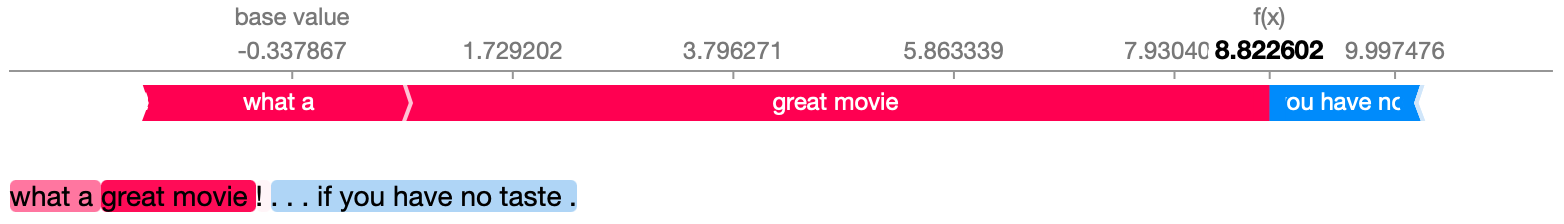
\includegraphics[width=\linewidth]{images/03_basics/sentiment_analysis_plot_movie.png}
    \caption{Linear approximation model \cite{shapDocs}}
    \label{fig:shapMovieExplained}
\end{figure}

Above we have an example of a linear explanation model, which provides the same result as the original model $f(x)$, but is much simpler to understand. The base value is the value you would get if you classified an empty text. The red text snippets are the words which move the classification score to a greater value, the blue ones to a lower value. At the end you get the same classification score as the classifier $f(x)$ produces.

\vspace{2cm}

The tool we implemented provides a post-hoc local explanation. We will now go into detail how it achieves that.